\documentclass{article}

\usepackage[spanish]{babel}

\usepackage[letterpaper,top=2cm,bottom=2cm,left=3cm,right=3cm,marginparwidth=1.75cm]{geometry}

\usepackage{amsmath}
\usepackage{graphicx}
\usepackage[colorlinks=true, allcolors=blue]{hyperref}

\title{Introducción a \LaTeX{}}
\author{Vladimir Piñera Verdecia}

\begin{document}
\maketitle

\begin{abstract}
Aquí se ubicaría el \emph{abstract}, el cual es un resumen breve, objetivo y preciso del contenido más relevante de un documento académico o científico. Se utiliza en textos académicos como artículos, ensayos, tesis, reportes técnicos e informes.
\end{abstract}

\section{Introducción}

LaTeX es un sistema de preparación de documentos para la composición de textos de alta calidad tipográfica1. Es utilizado principalmente para documentos técnicos o científicos de tamaño mediano a grande, pero puede ser utilizado para casi cualquier forma de publicación1. LaTeX no es un procesador de texto como Microsoft Word o Google Docs.

LaTeX se utiliza para crear documentos que contienen texto y fórmulas matemáticas con calidad de imprenta. Es especialmente útil para la generación de artículos y libros científicos que incluyen expresiones matemáticas.

Es un sistema de composición muy adecuado para realizar textos científicos y matemáticos de alta calidad tipográfica. Además, es adecuado para producir documentos de cualquier otro tipo, desde simples cartas hasta libros enteros.

\section{Algunos ejemplos para empezar}

\subsection{Como crear secciones y subsecciones}

Basta con utilizar los comandos de \emph{section} y \emph{subsection}, como en este documento de ejemplo.

\subsection{Cómo incluir imágenes}

Primero, debes tener en el mismo directorio donde se ubica este archivo, la imagen que se quiere agregar. Usa el entorno \emph{figure} para insertar imágenes. A continuación, utiliza el comando \emph{includegraphics} para incluirla en tu documento, también debe añadir un caption.
Ten en cuenta que su imagen se colocará automáticamente en el lugar más apropiado para ella, teniendo en cuenta el texto circundante y otras imágenes o tablas que puedan estar cerca.

\begin{figure}
\centering
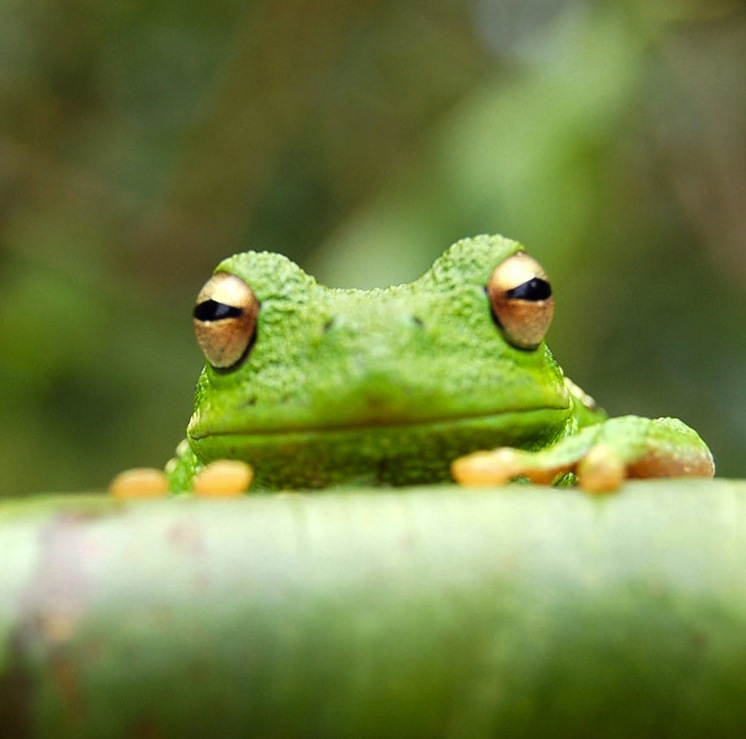
\includegraphics[width=0.25\linewidth]{frog.jpg}
\caption{\label{fig:frog}Rana.}
\end{figure}

\subsection{Cómo añadir tablas}

Utiliza los entornos \emph{table} y \emph{tabular} para crear tablas

\begin{table}
\centering
\begin{tabular}{l|r}
Tipo de Rana & Esperanza de Vida (años) \\\hline
Arbórea & 5-6  \\
Toro & 10-15
\end{tabular}
\caption{\label{tab:widgets}Tabla de ejemplo.}
\end{table}

\subsection{Cómo añadir comentarios}

Para agregar comentarios en código LaTeX usa \%

\subsection{Cómo añadir listas}

Puedes crear listas con numeración automática:

\begin{enumerate}
\item Rana1,
\item Rana2.
\end{enumerate}
o con puntos:
\begin{itemize}
\item Rana1,
\item Rana2.
\end{itemize}

Estas listas se crean con los entornos \emph{enumerate} y \emph{itemize}.

\subsection{Cómo escribir fórmulas matemáticas}

\LaTeX{} is great at typesetting mathematics. Let $X_1, X_2, \ldots, X_n$ be a sequence of independent and identically distributed random variables with $\text{E}[X_i] = \mu$ and $\text{Var}[X_i] = \sigma^2 < \infty$, and let
\[S_n = \frac{X_1 + X_2 + \cdots + X_n}{n}
      = \frac{1}{n}\sum_{i}^{n} X_i\]
denote their mean. Then as $n$ approaches infinity, the random variables $\sqrt{n}(S_n - \mu)$ converge in distribution to a normal $\mathcal{N}(0, \sigma^2)$.

\subsection{How to add Citations and a References List}

You can simply upload a \verb|.bib| file containing your BibTeX entries, created with a tool such as JabRef. You can then cite entries from it, like this: \cite{greenwade93}. Just remember to specify a bibliography style, as well as the filename of the \verb|.bib|. You can find a \href{https://www.overleaf.com/help/97-how-to-include-a-bibliography-using-bibtex}{video tutorial here} to learn more about BibTeX.

If you have an \href{https://www.overleaf.com/user/subscription/plans}{upgraded account}, you can also import your Mendeley or Zotero library directly as a \verb|.bib| file, via the upload menu in the file-tree.

\subsection{Good luck!}

We hope you find Overleaf useful, and do take a look at our \href{https://www.overleaf.com/learn}{help library} for more tutorials and user guides! Please also let us know if you have any feedback using the Contact Us link at the bottom of the Overleaf menu --- or use the contact form at \url{https://www.overleaf.com/contact}.

\bibliographystyle{alpha}
\bibliography{sample}

\end{document}